\documentclass{article}
\title{\textbf{Laboratorio 07 \\ Uno a muchos, muchos a muchos, email y PDF}}
\author{Melsy Melany Huamaní Vargas}

\usepackage{fancyhdr}
\usepackage{graphicx}
\usepackage{geometry}
\geometry{top=3cm,a4paper,right=2.5cm}
\usepackage{hyperref}

\usepackage[utf8]{inputenc}
\usepackage[T1]{fontenc}
\usepackage[spanish]{babel}
\usepackage{times}

\usepackage{color}
\definecolor{gray97}{gray}{.97}
\definecolor{gray75}{gray}{.75}
\definecolor{gray45}{gray}{.45}

\usepackage{listings}
\lstset{ frame=Ltb,
framerule=0pt,
aboveskip=0.5cm,
framextopmargin=3pt,
framexbottommargin=3pt,
framexleftmargin=0.4cm,
framesep=0pt,
rulesep=.4pt,
backgroundcolor=\color{gray97},
rulesepcolor=\color{black},
%
stringstyle=\ttfamily,
showstringspaces = false,
basicstyle=\small\ttfamily,
commentstyle=\color{gray45},
keywordstyle=\bfseries,
%
numbers=left,
numbersep=15pt,
numberstyle=\tiny,
numberfirstline = false,
breaklines=true,
%
xleftmargin=30pt,
}

\lstnewenvironment{listing}[1][]
{\lstset{#1}\pagebreak[0]}{\pagebreak[0]}

\lstdefinestyle{shell}
{basicstyle=\scriptsize\bf\ttfamily,
backgroundcolor=\color{gray75},
language=sh,
numbers=none,
}

\lstdefinestyle{python}
{language=python,
}

\lstdefinestyle{html}
{language=html,
}

\pagestyle{fancy}
\fancyhf{}
\fancyhead[L]{\includegraphics[height=1cm]{imagenes/epis.png}}
\fancyhead[C]{\fontsize{7}{8}\selectfont
\begin{tabular}{c}
  UNIVERSIDAD NACIONAL DE SAN AGUSTIN \\
  FACULTAD DE INGENIERÍA DE PRODUCCIÓN Y SERVICIOS \\
  DEPARTAMENTO ACADÉMICO DE INGENIERÍA DE SISTEMAS E INFORMÁTICA \\
  ESCUELA PROFESIONAL DE INGENIERÍA DE SISTEMAS
\end{tabular}}
\fancyhead[R]{\includegraphics[height=1cm]{imagenes/abet.png}}


\usepackage{xcolor}
\usepackage{colortbl}
\usepackage{array}

\setlength{\headheight}{2cm}

\begin{document}

\begin{titlepage}
  \maketitle 

  \vspace{2cm}
  
  \begin{center}
    \begin{tabular}{|>{\centering\arraybackslash}p{3cm}|>{\centering\arraybackslash}p{3cm}|>{\centering\arraybackslash}p{3cm}|}
      \hline
      \rowcolor{red}
      \textcolor{white}{Profesor} & \textcolor{white}{Escuela} & \textcolor{white}{Asignatura} \\
      \hline
      Anibal Sardon Paniagua & Ingeniería de Sistemas & Programación Web 2 \\
      \hline
    \end{tabular}
  \end{center}

  \vspace{5pt}

  \begin{center}
    \begin{tabular}{|>{\centering\arraybackslash}p{3cm}|>{\centering\arraybackslash}p{3cm}|>{\centering\arraybackslash}p{3cm}|}
      \hline
      \rowcolor{red}
      \textcolor{white}{Laboratorio} & \textcolor{white}{Tema} & \textcolor{white}{Duración} \\
      \hline
      07 & Uno a muchos, mucho a muchos, email y pdf & 04 horas \\
      \hline
    \end{tabular}
  \end{center}

  \vspace{5pt}

  \begin{center}
    \begin{tabular}{|>{\centering\arraybackslash}p{3cm}|>{\centering\arraybackslash}p{3cm}|>{\centering\arraybackslash}p{3cm}|}
      \hline
      \rowcolor{red}
      \textcolor{white}{Semestre académico} & \textcolor{white}{Fecha de inicio} & \textcolor{white}{Fecha de entrega} \\
      \hline
      2023 - A & 04/07/2023 & 14/07/2023 \\
      \hline
    \end{tabular}
  \end{center}
\end{titlepage}


\noindent
\section*{\centering DESARROLLO}

\vspace{2\baselineskip}

\textbf{ENLACE GITHUB Y GIT}

Este trabajo se está presentando en el Github: \url{https://github.com/mhuamanivar/PW2-HuamaniV-Lab07} y el .git es: \url{https://github.com/mhuamanivar/PW2-HuamaniV-Lab07.git}, además el video de flipgrip es el siguiente: \url{https://flip.com/s/Ms_fZ__6sTyz}.

\vspace{2\baselineskip}

\textbf{CREANDO PROYECTO E INSTALANDO}

Se utiliza el sistema Windows para instalar las herramientas necesarias y crear el proyecto. En este caso, se escogió una aplicación library para que se muestran libros.

\vspace{\baselineskip}

\begin{itemize}
\item Primero se verifica la versión de Python.

\begin{lstlisting}[style=shell]
C:\Users\melsy>mkvirtualenv my_env7
created virtual environment CPython3.11.1.final.0-64 in 3903ms
  creator CPython3Windows(dest=C:\Users\melsy\Envs\my_env7, clear=False, no_vcs_ignore=False, global=False)
  seeder FromAppData(download=False, pip=bundle, setuptools=bundle, wheel=bundle, via=copy, app_data_dir=C:\Users\melsy\AppData\Local\pypa\virtualenv)
    added seed packages: pip==23.1.2, setuptools==67.8.0, wheel==0.40.0
  activators BashActivator,BatchActivator,FishActivator,NushellActivator,PowerShellActivator,PythonActivator
\end{lstlisting}

\item Se instala Django y xhtml2pdf

\begin{lstlisting}[style=shell]
(my_env7) C:\Users\melsy>pip install django
(my_env7) C:\Users\melsy>pip install --pre xhtml2pdf
\end{lstlisting}

\item Se crea el proyecto dentro de la carpeta `projects` y dentro de esta se crea la aplicación `library` para usarla más adelante.

\begin{lstlisting}[style=shell]
(my_env7) C:\Users\melsy>cd projects
(my_env7) C:\Users\melsy\projects> django-admin startproject proyecto
(my_env7) C:\Users\melsy\projects>cd proyecto
(my_env7) C:\Users\melsy\projects\proyecto>python manage.py startapp library
\end{lstlisting}

\item Se corre el servidor y se puede ver lo siguiente

\begin{minipage}{\linewidth}
  \centering
  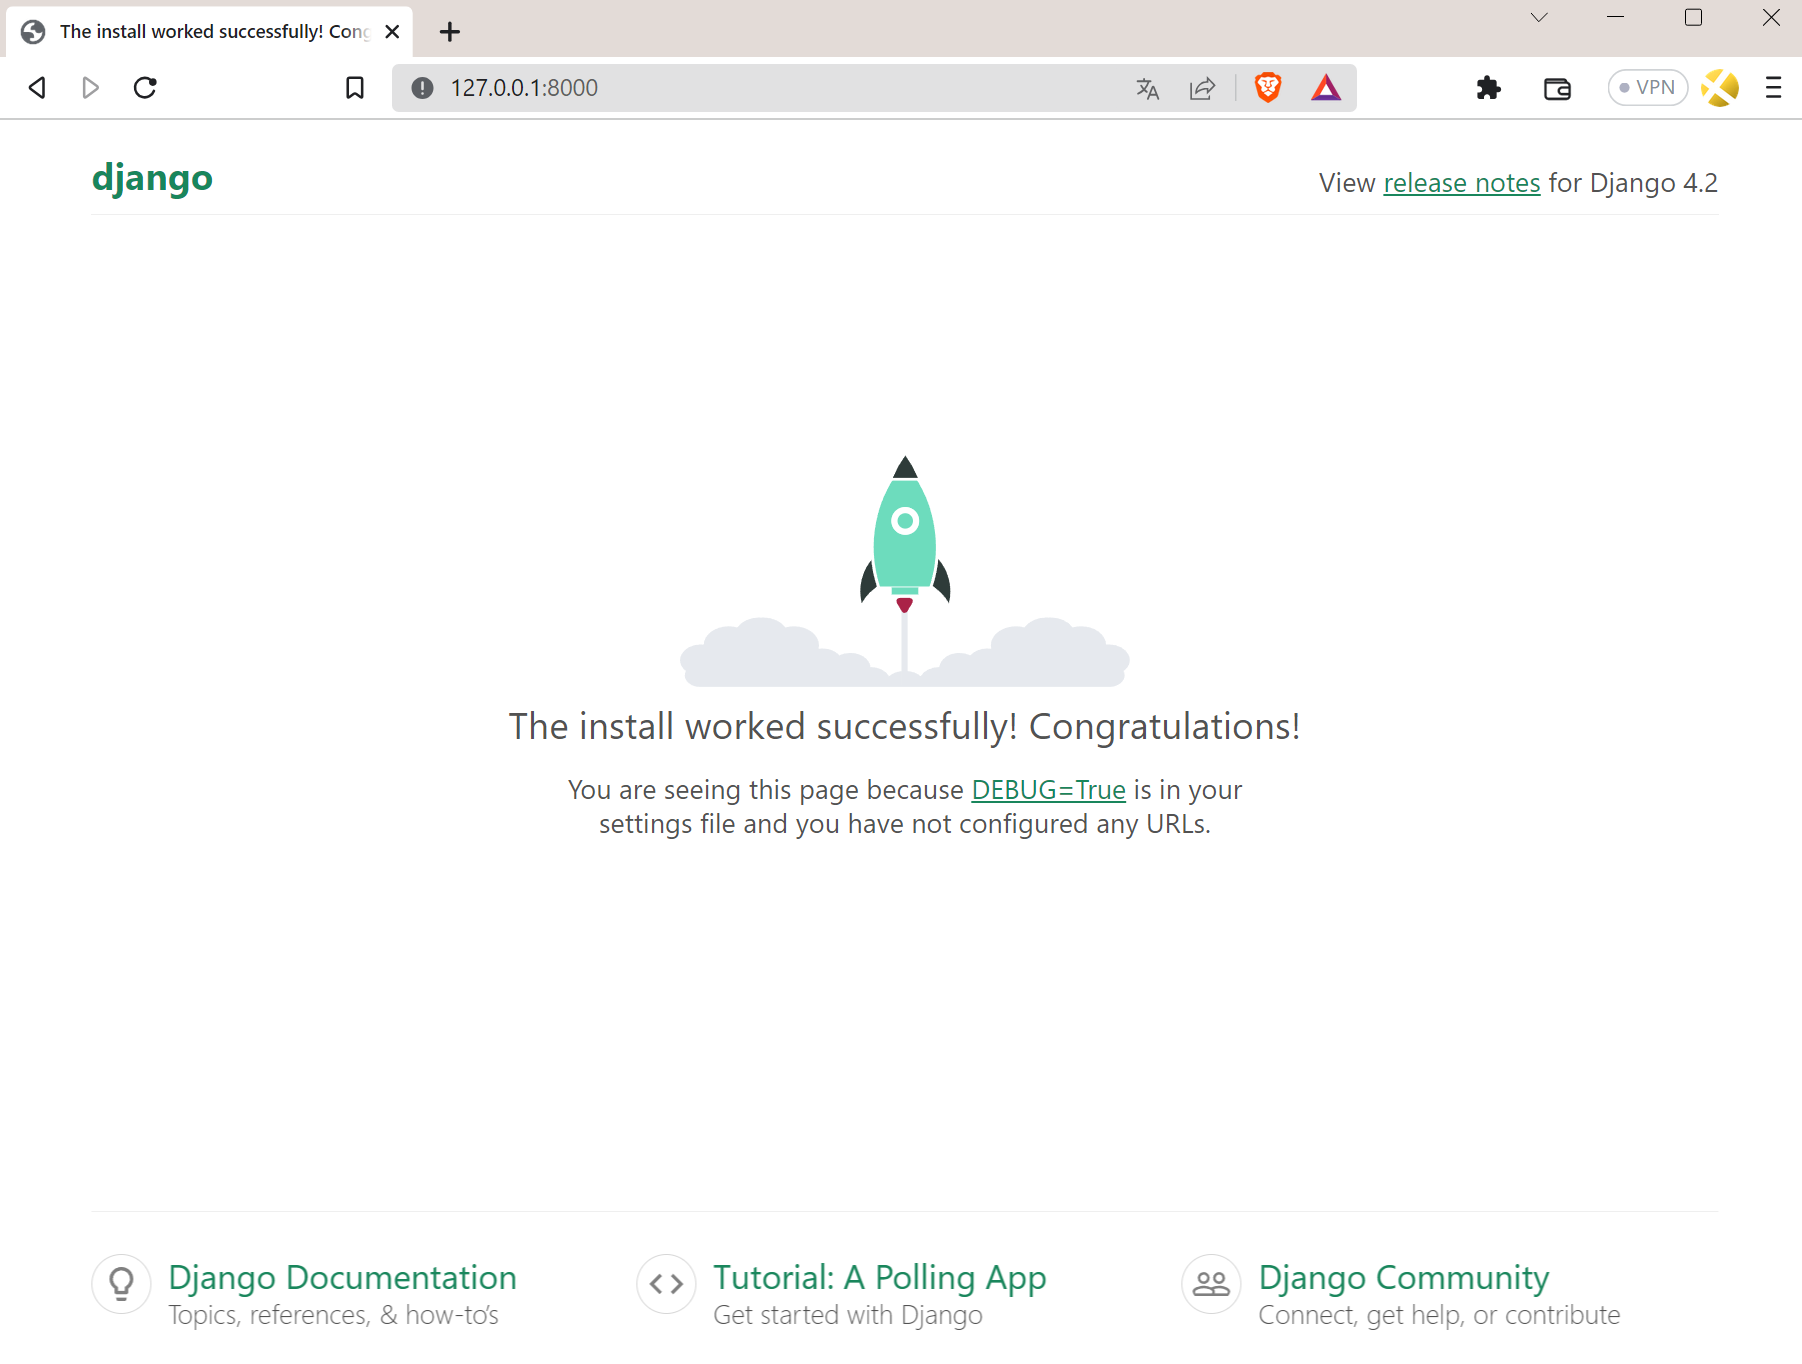
\includegraphics[width=0.90\textwidth]{imagenes/img1.png}
\end{minipage}

\end{itemize}

\vspace{2\baselineskip}

\textbf{CREANDO LOS MODELOS, UNO A MUCHOS Y MUCHOS A MUCHOS}

\vspace{\baselineskip}

\begin{itemize}
\item Primero se añade la aplicación creada en el archivo `settings.py` de `lab07`.

\begin{lstlisting}[style=python]
INSTALLED_APPS = [
    'django.contrib.admin',
    'django.contrib.auth',
    'django.contrib.contenttypes',
    'django.contrib.sessions',
    'django.contrib.messages',
    'django.contrib.staticfiles',
    'library' # Se agrega esta linea
]
\end{lstlisting}

\item Se crea el modelo `Author` que tiene relación de uno a muchos con el modelo `Book`.

\begin{lstlisting}[style=python]
class Author(models.Model):
    name = models.CharField(max_length=100)

    def __str__(self):
        return self.name
\end{lstlisting}

\item Ahora se crea el modelo `Publisher` que en este caso tiene relación de muchos a muchos con el modelo `Book`.

\begin{lstlisting}[style=python]
class Publisher(models.Model):
    name = models.CharField(max_length=100)

    def __str__(self):
        return self.name
\end{lstlisting}

\item Se tiene el modelo `Book` el cual tiene relación uno a muchos y muchos a muchos.

\begin{lstlisting}[style=python]
class Book(models.Model):
    title = models.CharField(max_length=100)
    author = models.ForeignKey(Author, on_delete=models.CASCADE)
    publisher = models.ManyToManyField(Publisher)
    summary = models.TextField()

    def __str__(self):
        return self.title
\end{lstlisting}

\item Se hacen las migraciones de los modelos del proyecto.

\begin{lstlisting}[style=shell]
(my_env7) C:\Users\melsy\projects\proyecto>python manage.py makemigrations
Migrations for 'library':
  library\migrations\0001_initial.py
    - Create model Author
    - Create model Publisher
    - Create model Book
(my_env7) C:\Users\melsy\projects\proyecto>python manage.py migrate
Operations to perform:
  Apply all migrations: admin, auth, contenttypes, library, sessions
Running migrations:
  Applying library.0001_initial... OK
\end{lstlisting}

\end{itemize}

\vspace{2\baselineskip}

\textbf{CONFIGURANDO VIEWS, EMAIL Y PDF}

\vspace{\baselineskip}

\begin{itemize}

\item Se crean las vistas para ver la lista de libro y los detalles del libro seleccionado en `views.py` de library.

\begin{lstlisting}[style=python]
from django.shortcuts import render
from .models import Book

def book_list(request):
    books = Book.objects.all()
    return render(request, 'library/book_list.html', {'books': books})

def book_detail(request, book_id):
    book = get_object_or_404(Book, id=book_id)
    return render(request, 'library/book_detail.html', {'book': book})
\end{lstlisting}

\item Se crea la función `generate\_pdf` para generar el PDF con los detalles de un libro y se agregan los siguientes import en `views.py` de library.

\begin{lstlisting}[style=python]
from django.shortcuts import render, get_object_or_404
from django.http import HttpResponse
from django.template.loader import get_template
from xhtml2pdf import pisa
from .models import Book

def generate_pdf(request, book_id):
    book = get_object_or_404(Book, id=book_id)
    template_path = 'library/invoice.html'
    context = {
        'book': book,
    }
    response = HttpResponse(content_type='application/pdf')
    response['Content-Disposition'] = 'attachment; filename="book_details.pdf"'

    template = get_template(template_path)
    html = template.render(context)

    pisa_status = pisa.CreatePDF(html, dest=response)
    if pisa_status.err:
        return HttpResponse('Error al generar el PDF', status=500)
    return response
\end{lstlisting}

\item Se crea la función `send\_email` en `views.py` de library, para enviar un email el cual utiliza la función anterior para enviar el PDF con los detalles del libro.

\begin{lstlisting}[style=python]
from django.shortcuts import render, get_object_or_404
from django.http import HttpResponse
from django.template.loader import get_template
from django.core.mail import EmailMessage
from xhtml2pdf import pisa
from .models import Book

def send_email(request, book_id):
    if request.method == 'POST':
        pdf = generate_pdf(request, book_id)
        email_address = request.POST.get('email')

        email = EmailMessage(
            'Detalles del libro',
            'Adjunto encontraras los detalles del libro en formato PDF.',
            'melsy@gmail.com',
            [email_address]
        )

        email.attach('book_details.pdf', pdf.getvalue(), 'application/pdf')
        email.send()

        return render(request, 'library/email_sent.html')
    
    book = get_object_or_404(Book, id=book_id)
    return render(request, 'library/book_detail.html', {'book': book})
\end{lstlisting}

\item En el archivo `settings.py` de proyecto se colocan las credenciales del email para enviar el correo, par esto se utilizó la página de `Mailtrap` el cual brinda estas credenciales para pruebas de correo.

\begin{lstlisting}[style=python]
EMAIL_BACKEND = 'django.core.mail.backends.smtp.EmailBackend'
EMAIL_HOST = 'sandbox.smtp.mailtrap.io'
EMAIL_PORT = 587
EMAIL_HOST_USER = 'bd45a037fa56d1'
EMAIL_HOST_PASSWORD = '9a7f42a21e19bf'
EMAIL_USE_TLS = True
EMAIL_USE_SSL = False
\end{lstlisting}

\end{itemize}


\vspace{2\baselineskip}

\textbf{CONFIGURANDO URLS}

\vspace{\baselineskip}

\begin{itemize}

\item Se colocan las urls de library en el archivo de `urls.py` de proyecto para que puedan ser reconocidas.

\begin{lstlisting}[style=python]
from django.contrib import admin
from django.urls import path, include

urlpatterns = [
    path('admin/', admin.site.urls),
    path('library/', include('library.urls')),
]
\end{lstlisting}

\item Se colocan las urls en el archivo de `urls.py` de library para que sean reconocidas posteriormente.

\begin{lstlisting}[style=python]
from django.urls import path
from . import views

app_name = 'library'

urlpatterns = [
    path('books/', views.book_list, name='book_list'),
    path('book/<int:book_id>/', views.book_detail, name='book_detail'),
    path('book/<int:book_id>/pdf/', views.generate_pdf, name='generate_pdf'),
    path('book/<int:book_id>/email/', views.send_email, name='send_email'),
]
\end{lstlisting}

\end{itemize}


\vspace{2\baselineskip}

\textbf{CREANDO LOS ARCHIVOS HTML}

\vspace{\baselineskip}

\begin{itemize}

\item En primer lugar, se modifica el archivo `settings.py` de proyecto para que reconozca los archivos html.

\begin{lstlisting}[style=python]
TEMPLATES = [
    {
        'BACKEND': 'django.template.backends.django.DjangoTemplates',
        'DIRS': [os.path.join(BASE_DIR, 'templates')], # Se agrega esta linea
        'APP_DIRS': True,
        'OPTIONS': {
            'context_processors': [
                'django.template.context_processors.debug',
                'django.template.context_processors.request',
                'django.contrib.auth.context_processors.auth',
                'django.contrib.messages.context_processors.messages',
            ],
        },
    },
]
\end{lstlisting}

\item Se crea el archivo `book\_list.html` con lo siguiente.
 
\begin{lstlisting}[style=html]
<!DOCTYPE html>
<html>
<head>
    <title>Lista de libros</title>
</head>
<body>
    <h1>Lista de libros</h1>
    <ul>
    
        <li><a href="">{{ book.title }}</a></li>
    
        <li>No hay libros disponibles.</li>
    
    </ul>
</body>
</html>
\end{lstlisting}

\item Se crea el archivo `book\_detail.html` con lo siguiente.

\begin{lstlisting}[style=html]
<!DOCTYPE html>
<html>
<head>
    <title>Detalles del libro</title>
</head>
<body>
    <h1>Detalles del libro</h1>
    <h2>{{ book.title }}</h2>
    <p>Autor: {{ book.author.name }}</p>
    <p>Publicado por:</p>
    <ul>
        
            <li>{{ publisher.name }}</li>
        
    </ul>
    <p>Resumen: {{ book.summary }}</p>
    <form action="" method="POST">
        
        <label for="email">Enviar PDF por email:</label><br>
        <input type="email" id="email" name="email"><br>
        <input type="submit" value="Enviar">
    </form>
    <a href="">Descargar en PDF</a>

</body>
</html>
\end{lstlisting}

\item Se crea el archivo `invoice.html` para mostrar en PDF el contenido requerido.

\begin{lstlisting}[style=html]
<!DOCTYPE html>
<html>
<head>
    <title>Detalles del libro</title>
    <style type="text/css">
        body {
            font-weight: 200;
            font-size: 14px;
        }
        .header {
            font-size: 20px;
            font-weight: 100;
            text-align: center;
            color: #007cae;
        }
        .title {
            font-size: 22px;
            font-weight: 100;
            padding: 10px 20px 0px 20px;  
        }
        .details {
            padding: 10px 20px 0px 20px;
            text-align: left !important;
        }
        .hrItem {
            border: none;
            height: 1px;
            color: #333;
            background-color: #fff;
        }
    </style>
</head>
<body>
    <div class='wrapper'>
        <div class='header'>
            <p class='title'>Detalles del libro</p>
        </div>
        <div class='details'>
            <p>Autor: {{ book.author.name }}</p>
            <p>Publicado por: 
            
                {{ publisher.name }}, 
            
                Sin publicaciones
            
            </p>
            <p>Resumen: {{ book.summary }}</p>
            <hr class='hrItem' />
        </div>
    </div>
</body>
</html>
\end{lstlisting}

\item Se crea el archivo `email\_sent.html` donde se confirma que el correo ha sido enviado.

\begin{lstlisting}[style=html]
<!DOCTYPE html>
<html>
<head>
    <title>Confirmacion de envio de correo</title>
</head>
<body>
    <h1>Correo electronico enviado</h1>
    <p>Se ha enviado el correo electronico con los detalles del libro en formato PDF.</p>
</body>
</html>
\end{lstlisting}

\end{itemize}


\vspace{2\baselineskip}

\textbf{CONFIGURANDO PAGINA DE ADMIN}

\vspace{\baselineskip}

\begin{itemize}

\item En primer lugar se modifica `admin.py` de library para que se puedan crear los modelos de author, book y publisher.

\begin{lstlisting}[style=python]
from django.contrib import admin
from .models import Book, Author, Publisher

@admin.register(Book)
class BookAdmin(admin.ModelAdmin):
    pass

@admin.register(Author)
class AuthorAdmin(admin.ModelAdmin):
    pass

@admin.register(Publisher)
class PublisherAdmin(admin.ModelAdmin):
    pass
\end{lstlisting}

\item Se crea el superusuario para acceder a la página del administrador.

\begin{lstlisting}[style=shell]
(my_env7) C:\Users\melsy\projects\proyecto>python manage.py createsuperuser
Username (leave blank to use 'melsy'): mhuamanivar
Email address: mhuamanivar@unsa.edu.pe
Password:
Password (again):
This password is too common.
This password is entirely numeric.
Bypass password validation and create user anyway? [y/N]: y
Superuser created successfully.
\end{lstlisting}

\end{itemize}


\vspace{2\baselineskip}

\pagebreak

\textbf{VIENDO PAGINA DE ADMIN}

\vspace{\baselineskip}

\begin{itemize}

\item Se va a la página del admin

\begin{minipage}{\linewidth}
    \centering
    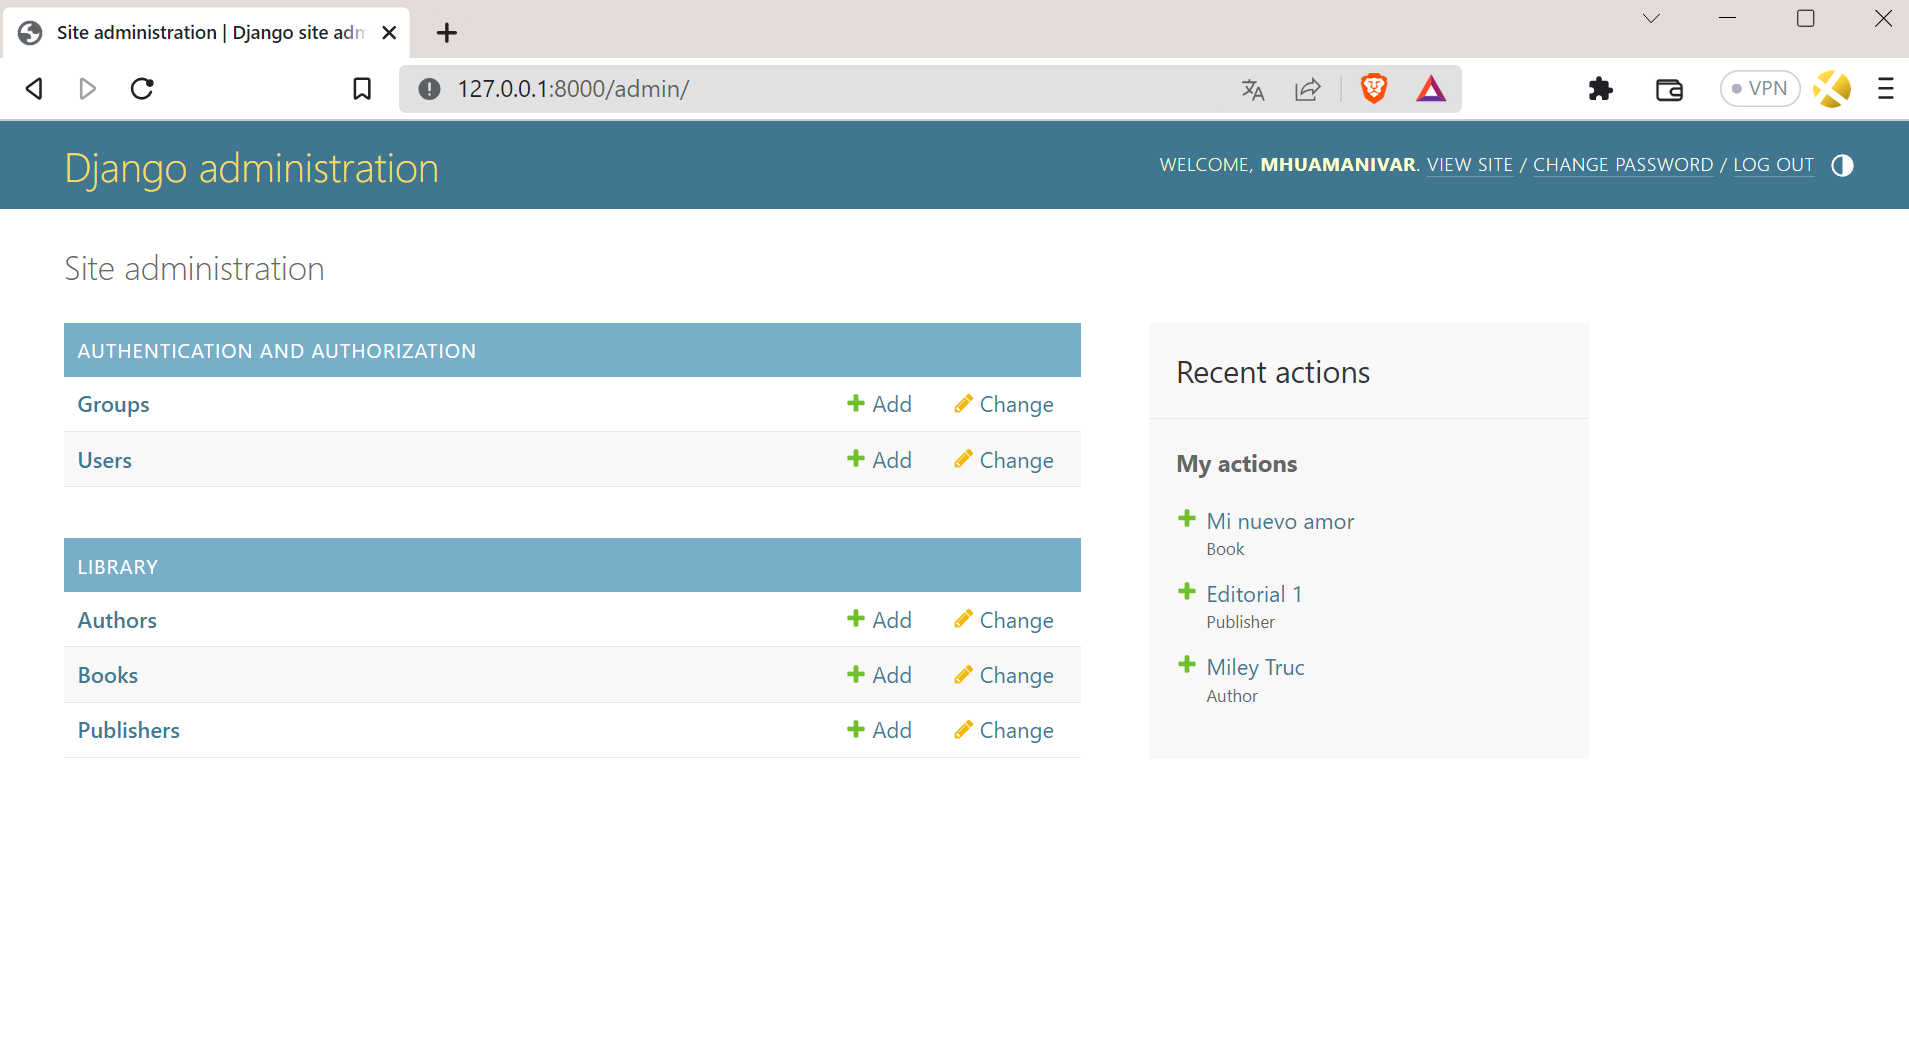
\includegraphics[width=0.90\textwidth]{imagenes/img2.png}
\end{minipage}
\vspace{\baselineskip}

\item Luego se da en `add` para añadir un libro, y colocamos los detalles importantes, se crea tres libros como ejemplo.

\begin{minipage}{\linewidth}
    \centering
    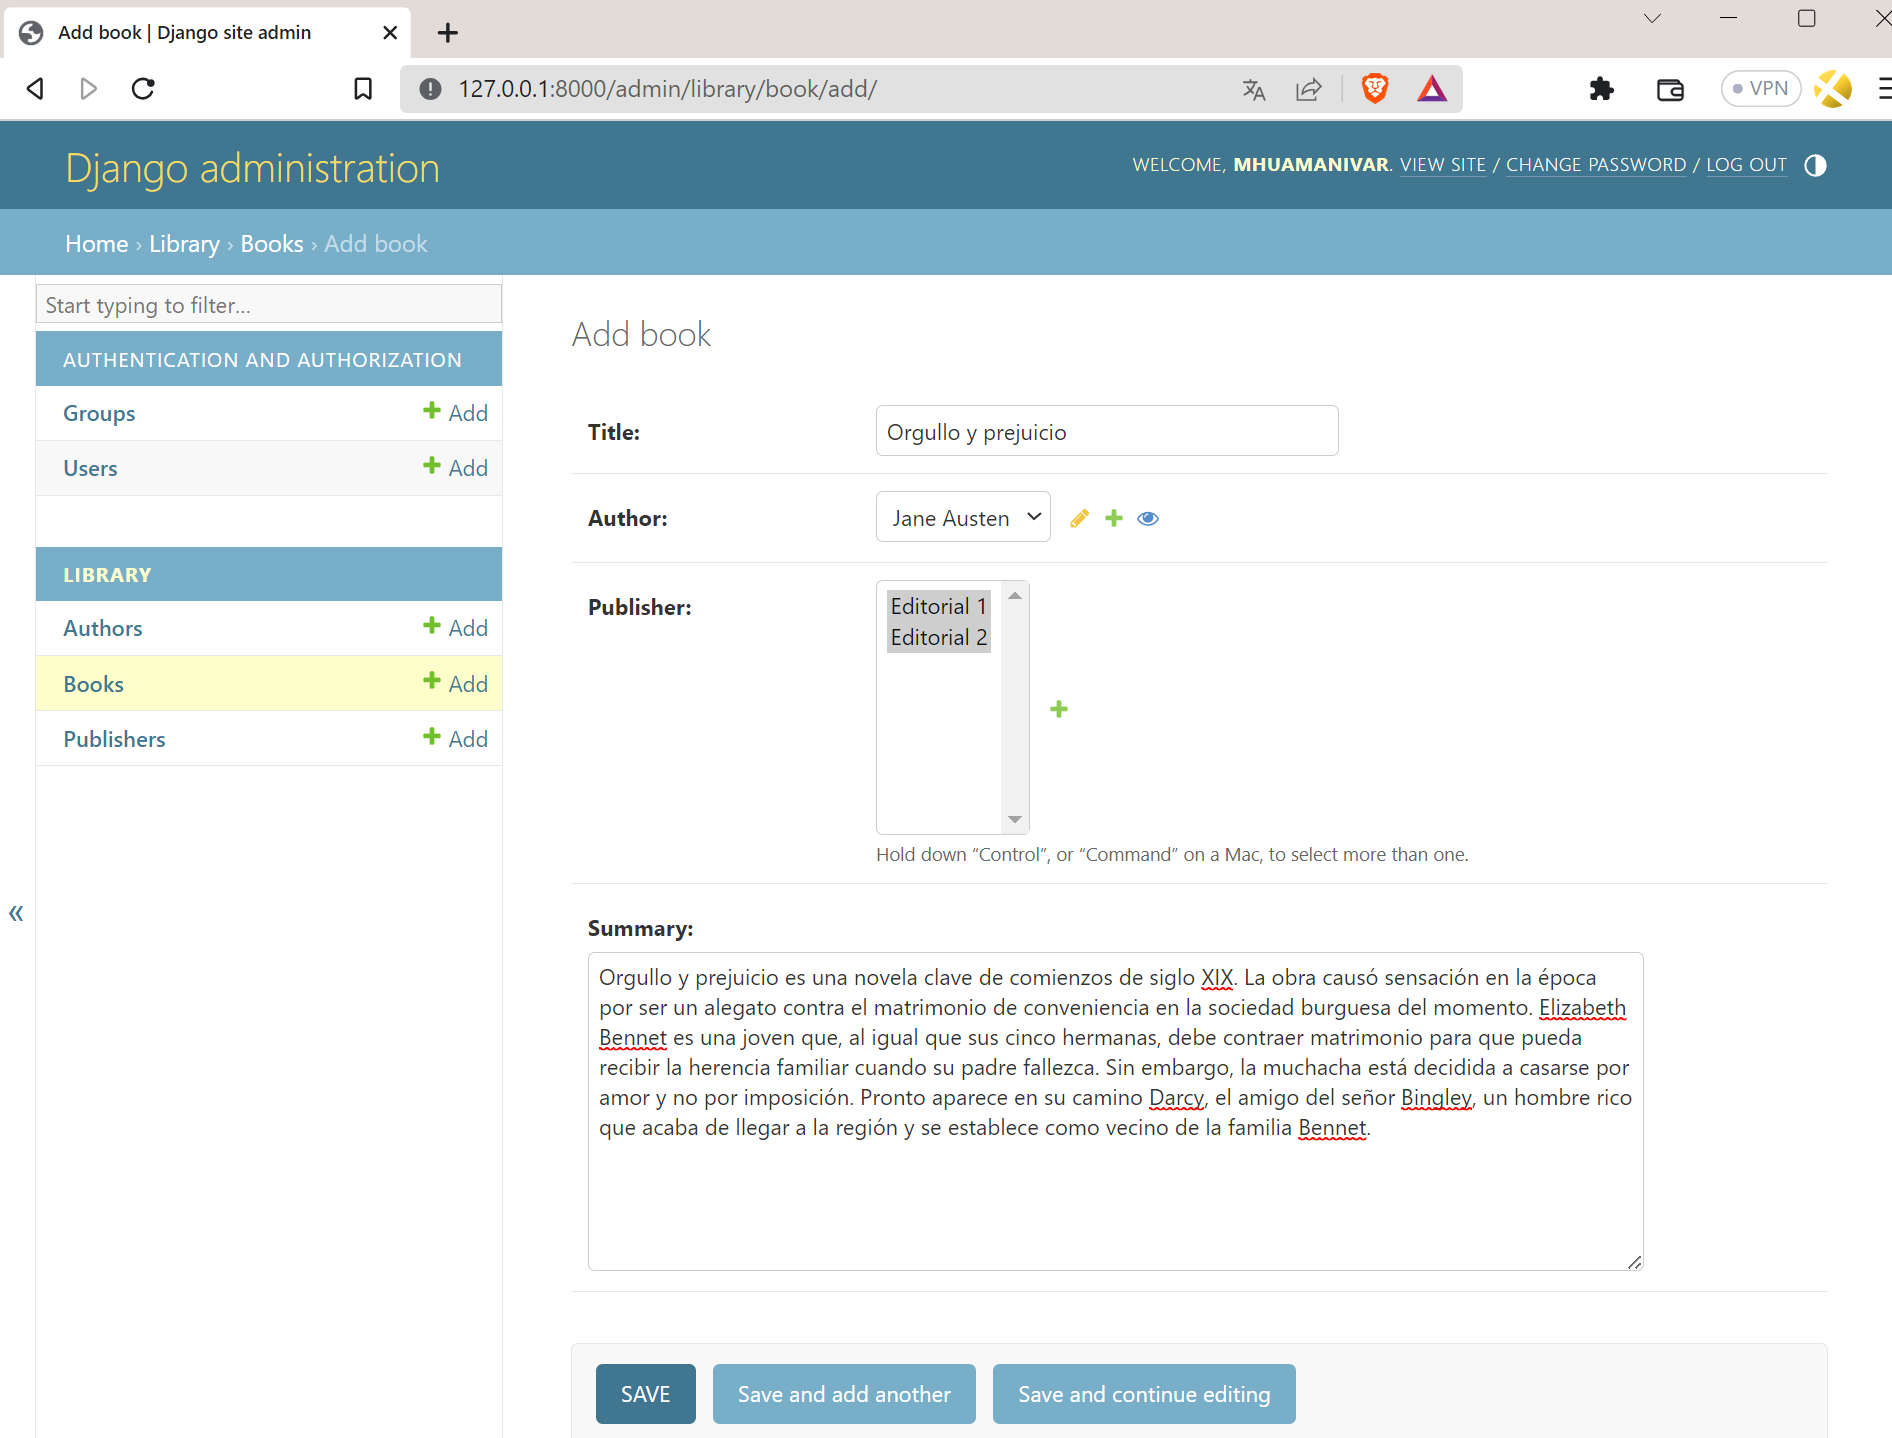
\includegraphics[width=0.90\textwidth]{imagenes/img3.png}
\end{minipage}
\vspace{\baselineskip}

\item Despues se puede ver la lista de libros creados en la pagina del admin.

\begin{minipage}{\linewidth}
    \centering
    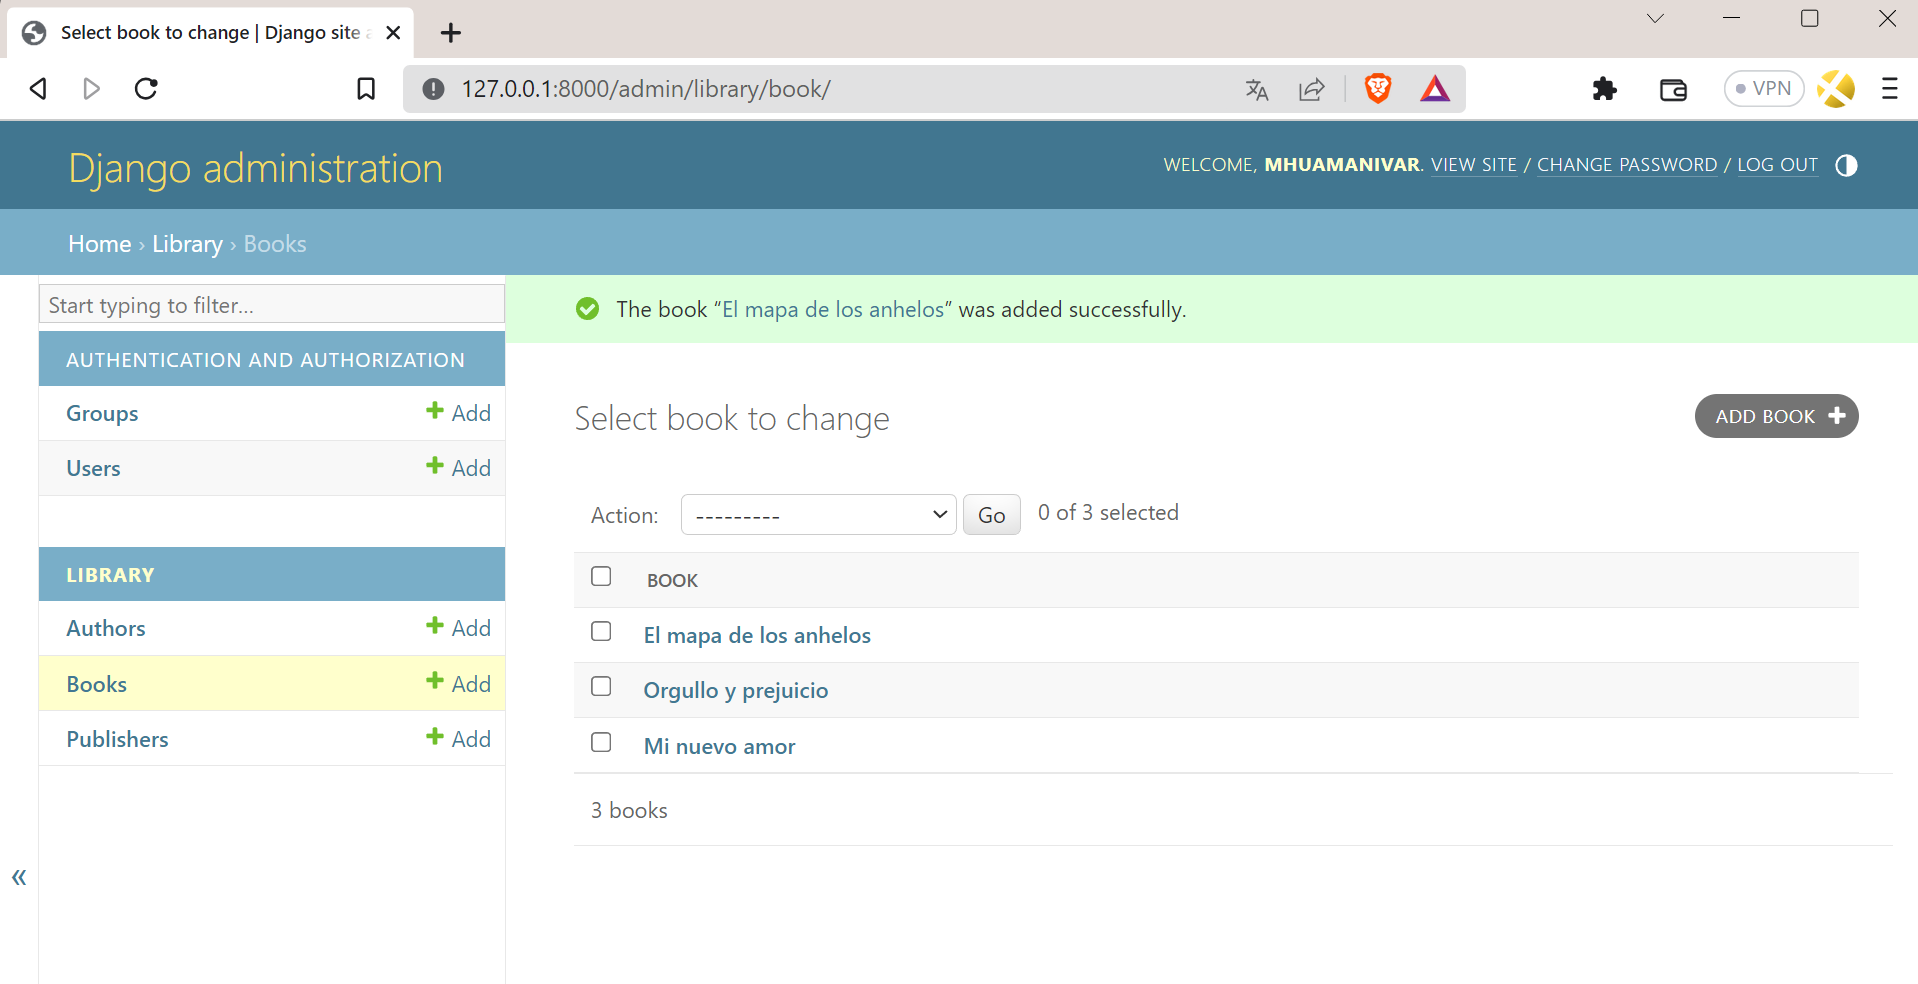
\includegraphics[width=0.90\textwidth]{imagenes/img4.png}
\end{minipage}
\vspace{\baselineskip}

\end{itemize}



\vspace{2\baselineskip}

\textbf{VIENDO LA PAGINA PRINCIPAL}

\vspace{\baselineskip}

\begin{itemize}

\item Se va a la pagina `http://127.0.0.1:8000/library/books/` y se ve la lista de libros

\begin{minipage}{\linewidth}
    \centering
    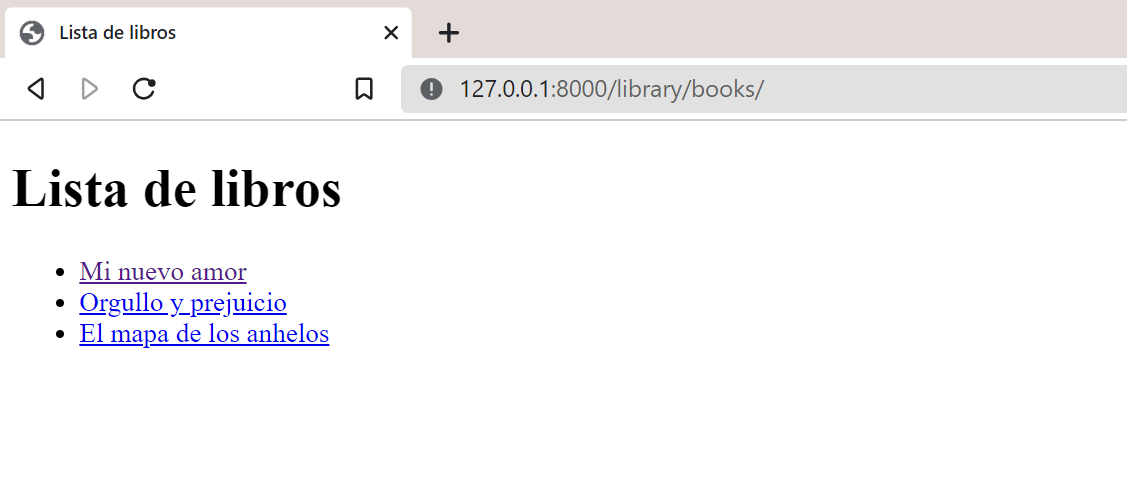
\includegraphics[width=0.90\textwidth]{imagenes/img5.png}
\end{minipage}
\vspace{\baselineskip}

\item Se da click a uno de ellos y se pueden ver los detalles del libro.

\begin{minipage}{\linewidth}
    \centering
    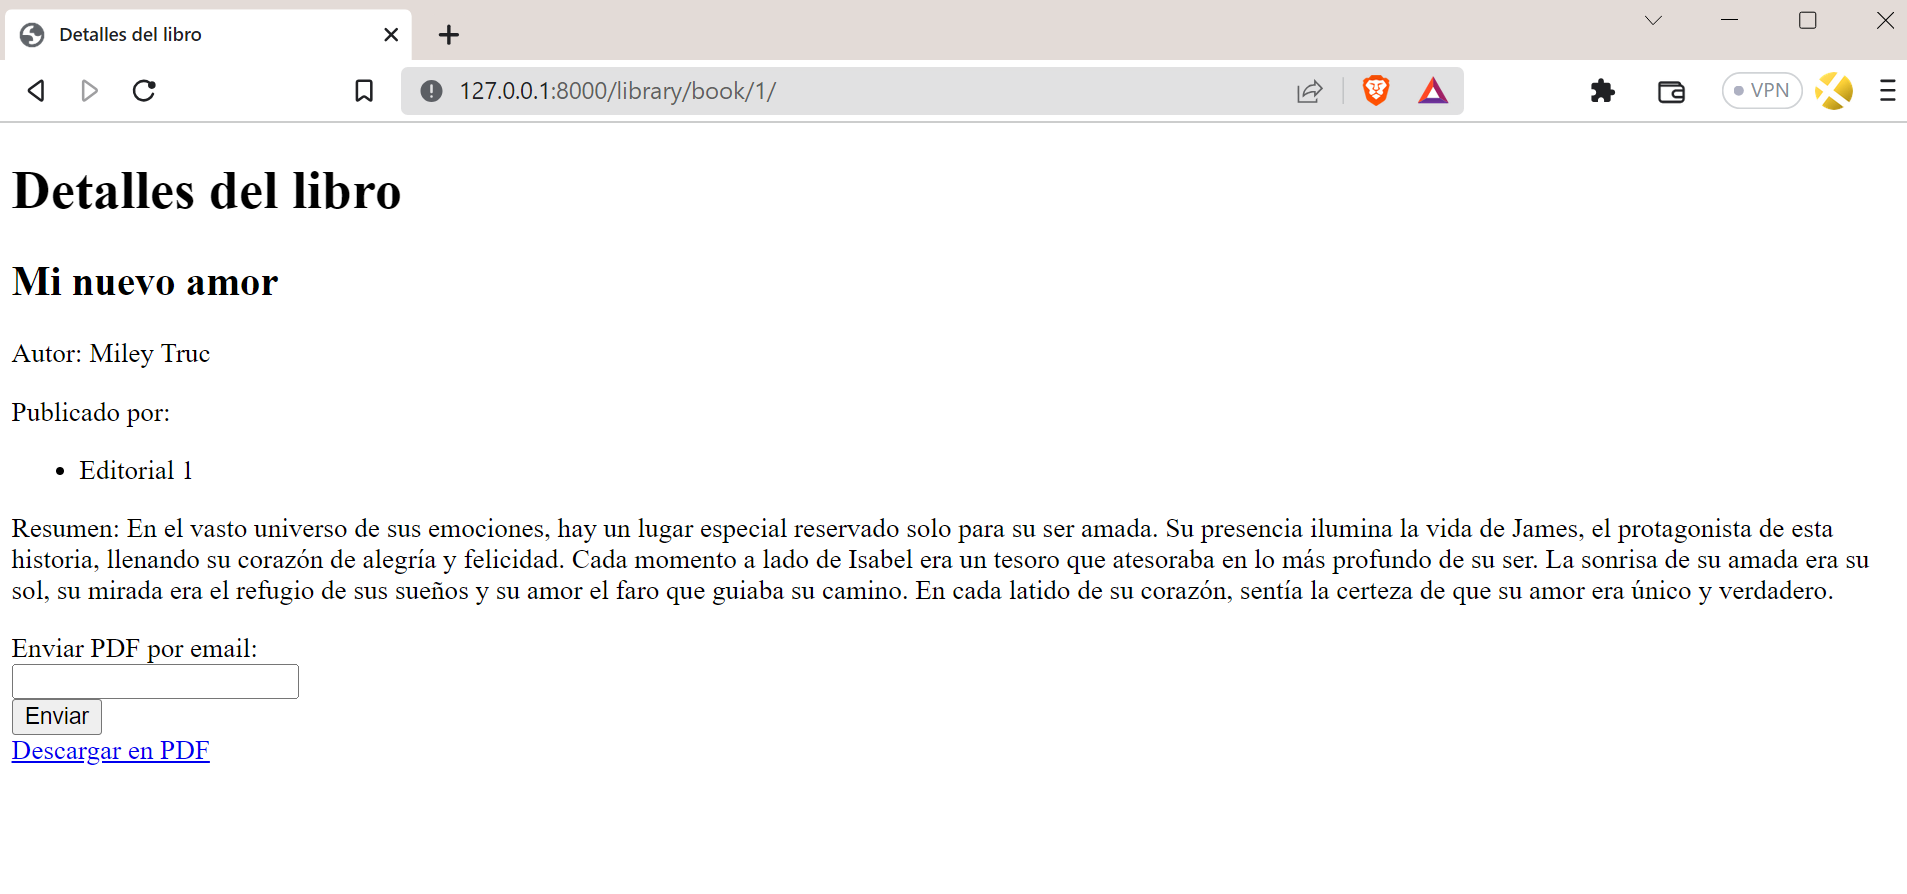
\includegraphics[width=0.90\textwidth]{imagenes/img6.png}
\end{minipage}
\vspace{\baselineskip}

\item Para enviar un correo, se inserta el correo al que se desea enviar

\begin{minipage}{\linewidth}
    \centering
    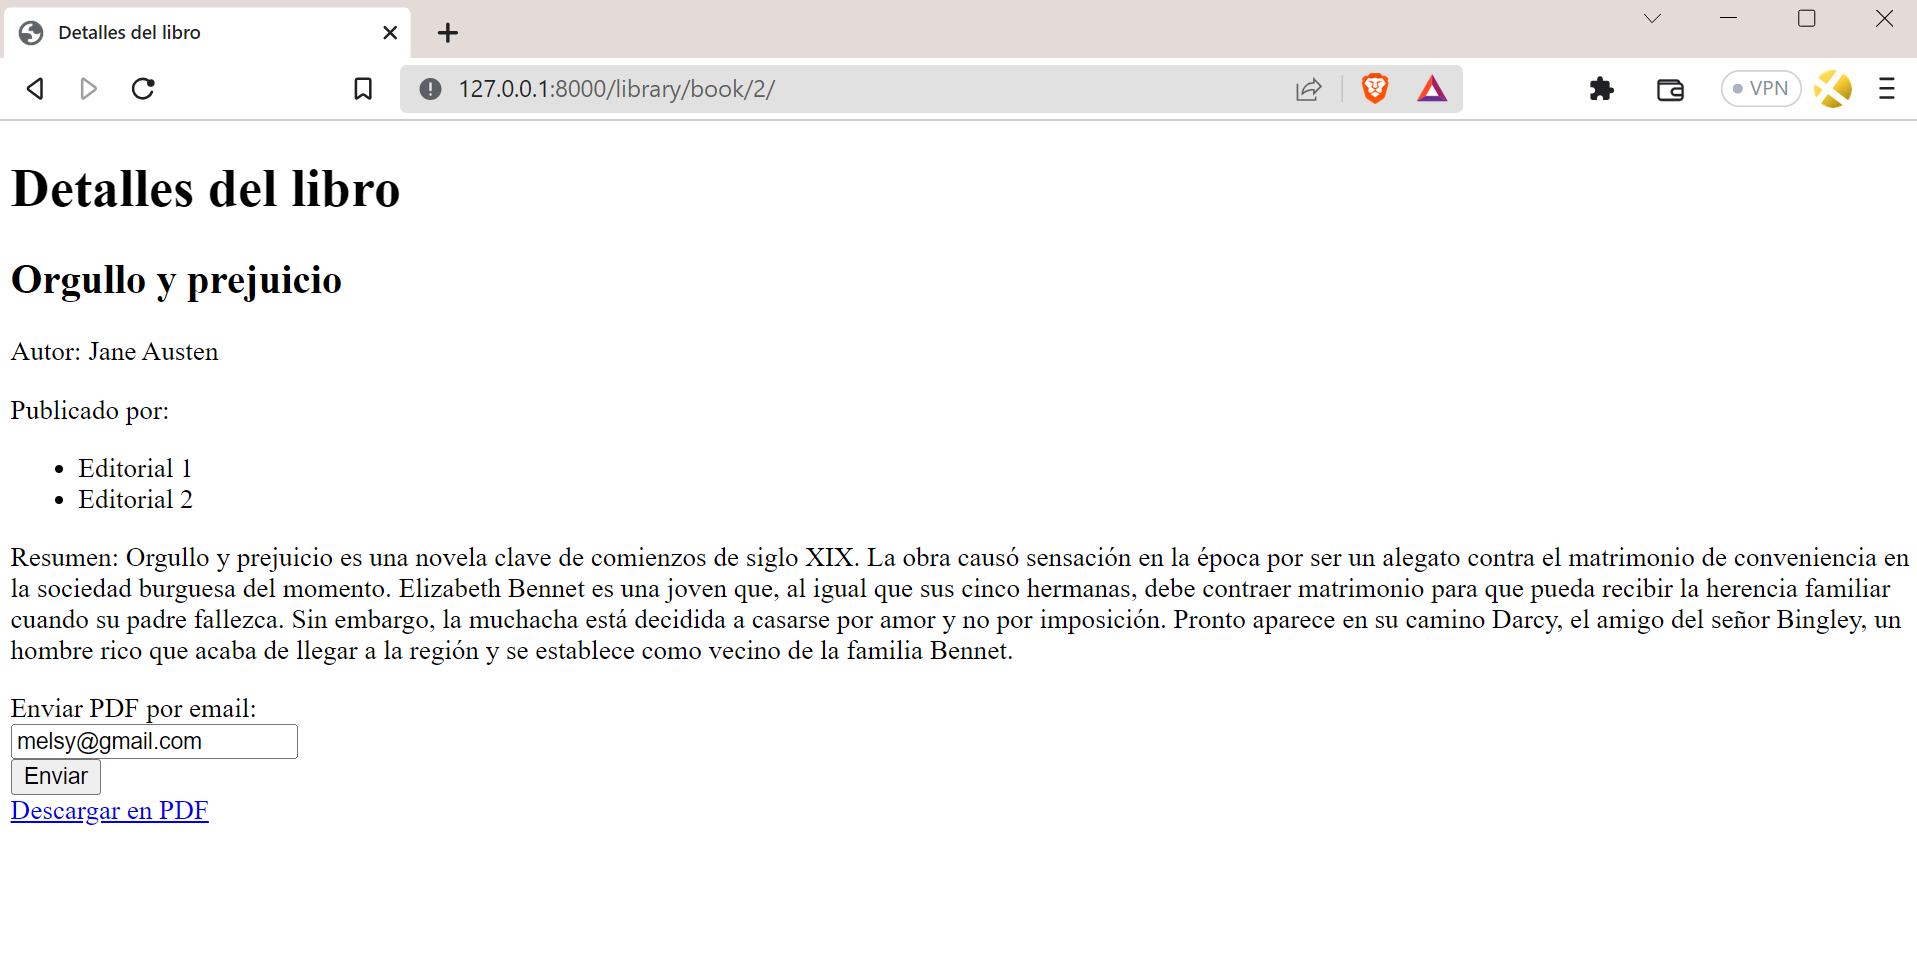
\includegraphics[width=0.90\textwidth]{imagenes/img7.png}
\end{minipage}
\vspace{\baselineskip}

\item Posteriormente se puede ver la pagina que menciona que se ha enviado correctamente.

\begin{minipage}{\linewidth}
    \centering
    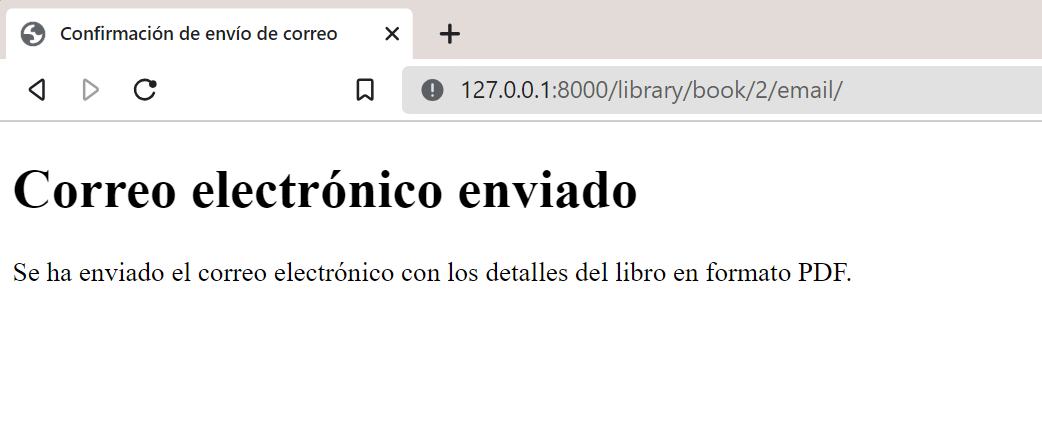
\includegraphics[width=0.70\textwidth]{imagenes/img8.png}
\end{minipage}
\vspace{\baselineskip}

\item Como se eligió trabajar con Mailtrap, entonces se va a la página y se puede ver que ha sido enviado correctamente el mensaje, además se ve de quien para quien va dirigido y el archivo que ha sido enviado en `Attachments`.

\begin{minipage}{\linewidth}
    \centering
    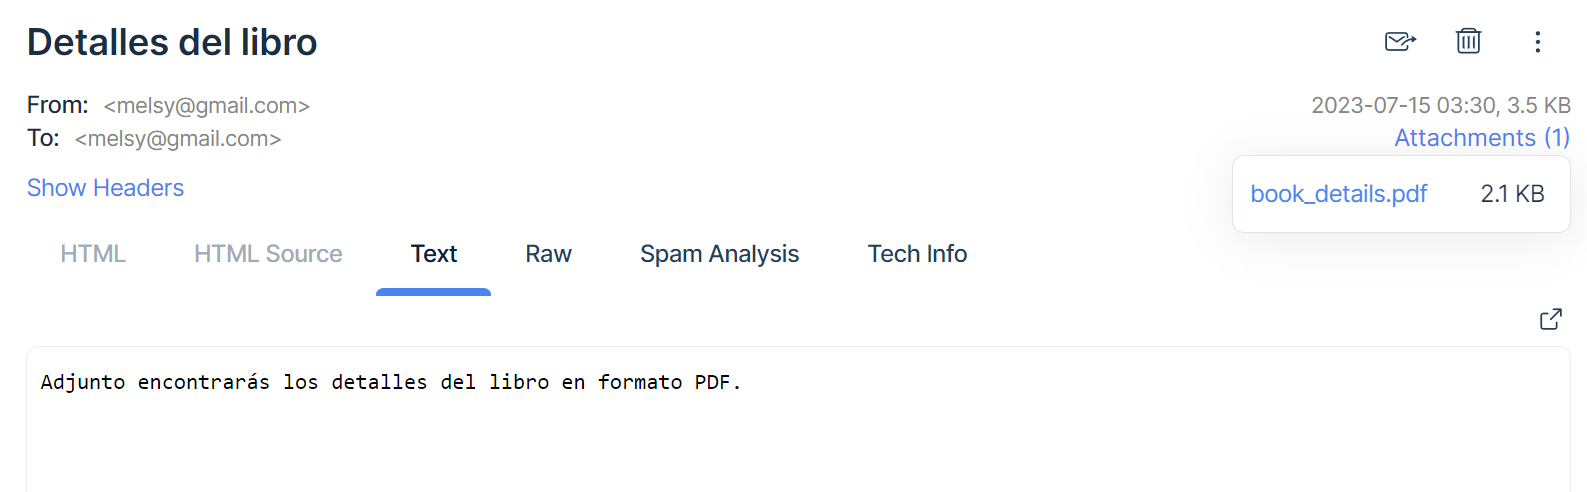
\includegraphics[width=0.90\textwidth]{imagenes/img9.png}
\end{minipage}
\vspace{\baselineskip}

\item Por otro lado, si se quiere enviar un PDF, entonces se hace click en `Descargar en PDF` y le damos en guardar en la carpeta que queremos.

\begin{minipage}{\linewidth}
    \centering
    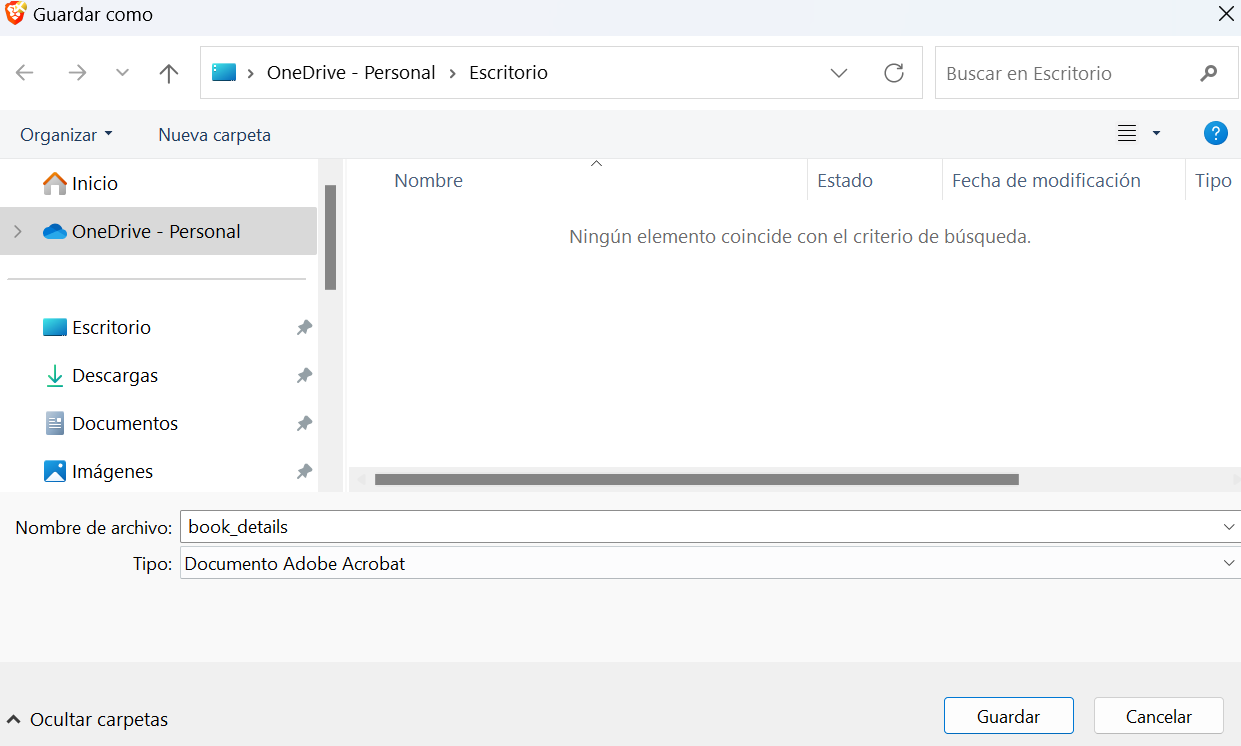
\includegraphics[width=0.90\textwidth]{imagenes/img10.png}
\end{minipage}
\vspace{\baselineskip}

\item Se confirma que ha sido guardado con el navegador.

\begin{minipage}{\linewidth}
    \centering
    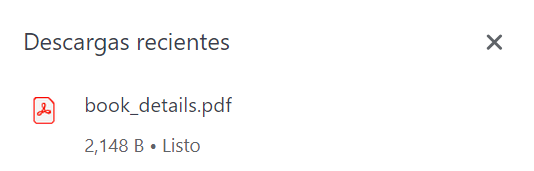
\includegraphics[width=0.70\textwidth]{imagenes/img11.png}
\end{minipage}
\vspace{\baselineskip}
\item Finalmente se puede ver el archivo en formato PDF, que contiene los detalles del libro.

\begin{minipage}{\linewidth}
    \centering
    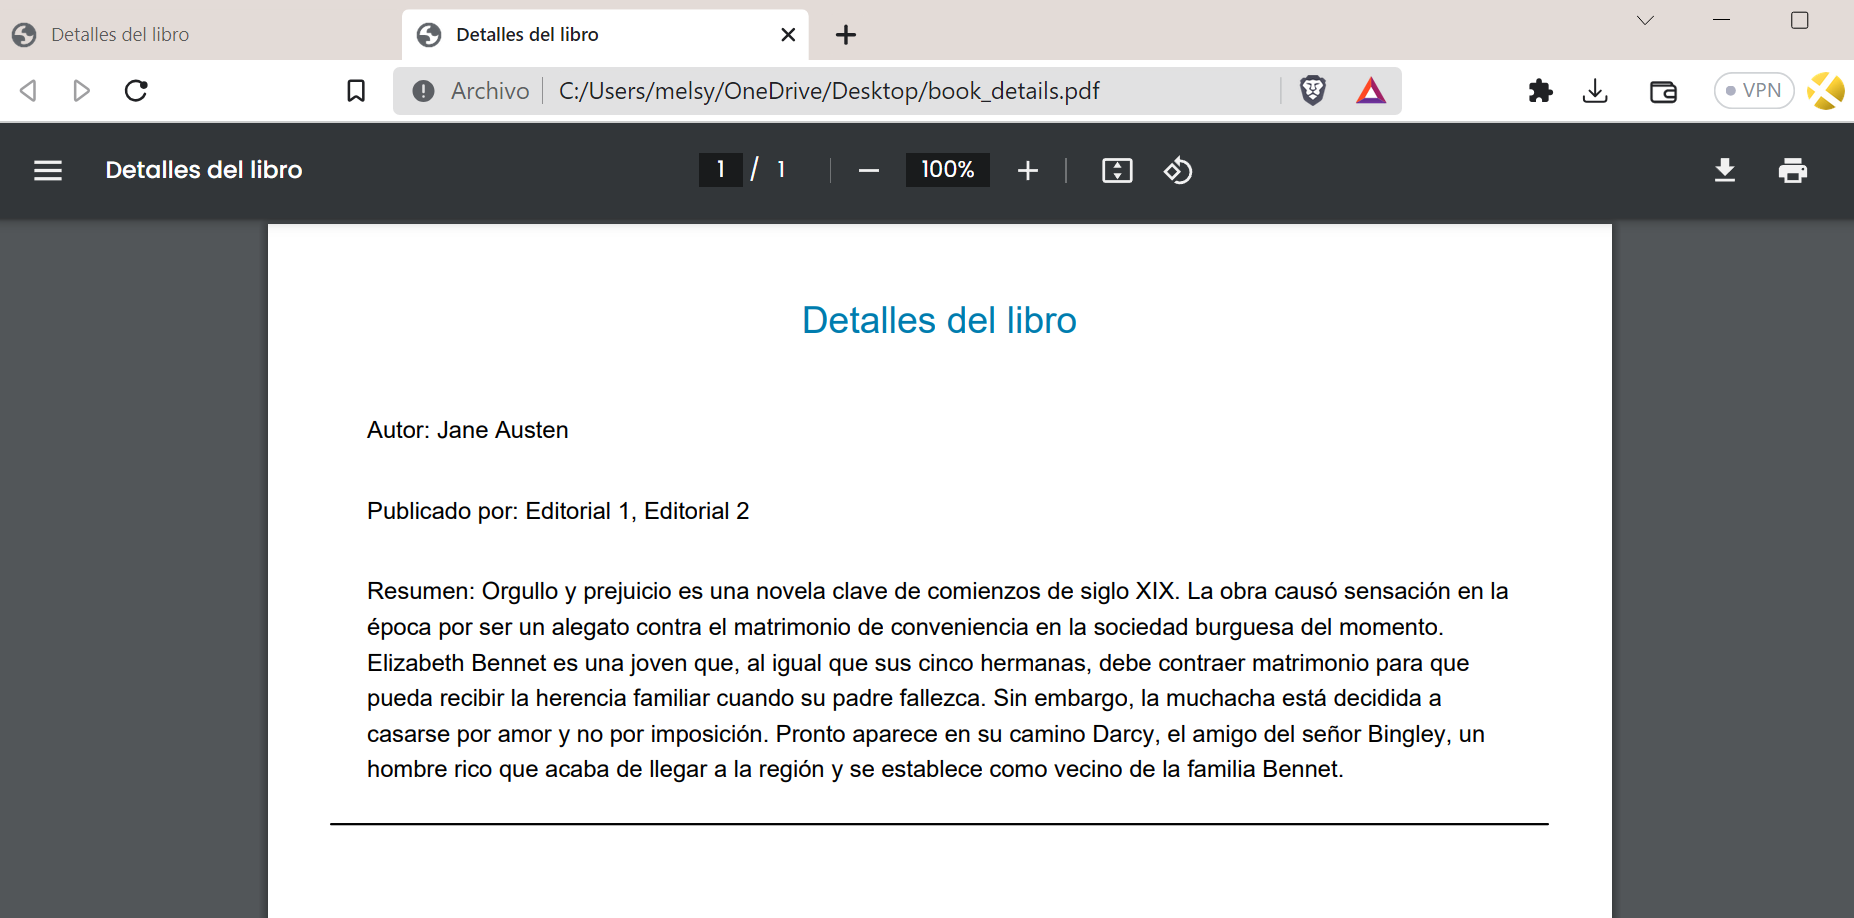
\includegraphics[width=0.90\textwidth]{imagenes/img12.png}
\end{minipage}

\end{itemize}

\end{document}